\documentclass[9pt]{extarticle}
\usepackage{amsmath}
\usepackage{bm}
\usepackage{graphicx}
\usepackage[utf8]{inputenc}
\usepackage{caption}
\usepackage{subcaption}
\title{Finite Element Method}
\author{Student \# }

\begin{document}
\maketitle

\section{Introduction}



The linear elasticity equation

\begin{equation}
\label{eq:linEl}
\nabla \bm{\sigma}(\bm{u}) = - \bm{f}.
\end{equation}

describes deformation and motion on a solid object. In this report, we will present how the linear elasticity equation is applied to a geometry in 3D using the finite element method. We will look at the convergence rate on our methods, and visualize how a bridge is deformed when a car drives over it. We will also look at stress on the bridge and explain parts of our algorithm.

General model, equation

% 2D problem:

Present the model, matrices
Displacement
Convergence

\subsection{Convergence analysis}

We test our code on the problem 

\begin{align}
f_x = \frac{E}{1-\nu^2} (-2y^2 - x^2 + \nu x^2 - 2\nu xy -2xy + 3 - \nu) \\
f_y = \frac{E}{1-\nu^2} (-2x^2 - y^2 + \nu y^2 - 2\nu xy -2xy + 3 - \nu) 
\end{align}

with homogeneous Dirichlet boundary conditions on all boundaries. Compared to the analytical solution 

\begin{align}
\bm{u}(x,y) = \begin{bmatrix}
\, (x^2-1)(y^2-1) \, \\
(x^2-1)(y^2-1)
\end{bmatrix}
\end{align}

we get the error plot shown in Figure \ref{error}. Also, increasing the grid size in each spatial direction by a factor 2, we obtain an accuracy convergence of order 2, as shown in Figure \ref{convergence}. This implies that our code is correct.

\begin{figure}
\center
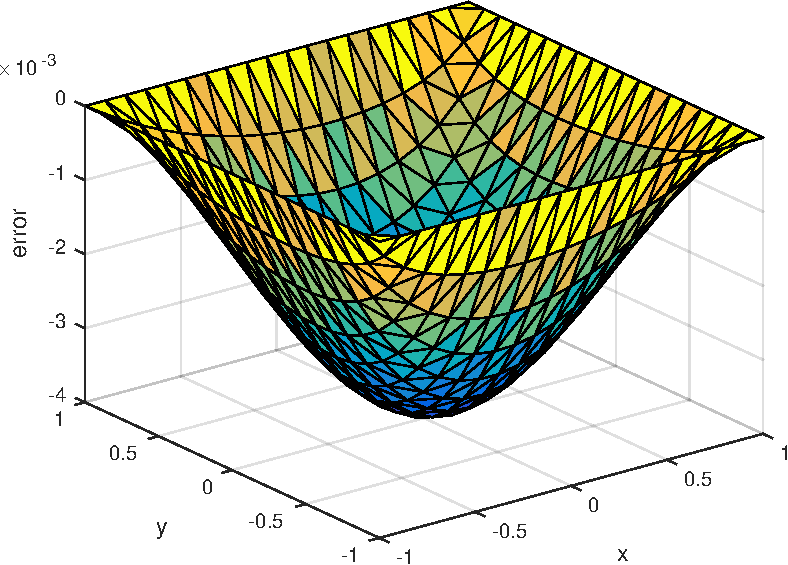
\includegraphics[width=0.4\textwidth]{error_linEl}
\caption{Error between the numerical solution to the linear elasticity problem and the analytical solution with $N = 20$ grid points in each spatial direction. The numerical solution is smaller than the analytical solution.}
\label{error}
\end{figure}

\begin{figure}[ht]
\center
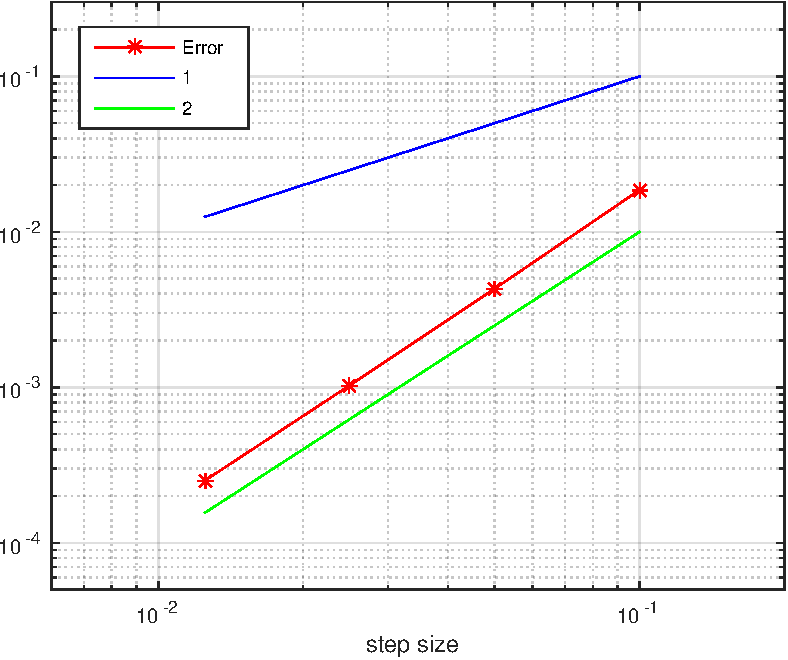
\includegraphics[width=0.4\textwidth]{conv_linEl}
\caption{Loglog plot of the error showing convergence of order 2 of the linear elasticity problem with $N =$ 10, 20, 40 and 80 grid points in each spatial direction. }
\label{convergence}
\end{figure}





% 3D problem:
Same shit as 2D

Present the model, matrices
Convergence


\subsection{Convergence analysis in 3D}

Inspired by the convergence test in 2D we test our code on the problem 

\begin{align}
f_x = &K^* \left[-2(y^2-1)(z^2-1) + (2 \nu -1)(x^2-1)(z^2 +y^2-2) \right.\nonumber\\
 &\left. -2x(y(z^2-1) + z(y^2-1)) \right] \\
 f_y = &K^* \left[-2(x^2-1)(z^2-1) + (2 \nu -1)(y^2-1)(z^2 +x^2-2) \right.\nonumber\\
 &\left. -2y(x(z^2-1) + z(x^2-1)) \right] \\
 f_z = &K^* \left[-2(x^2-1)(y^2-1) + (2 \nu -1)(z^2-1)(y^2 +x^2-2) \right.\nonumber\\
 &\left. -2z(x(y^2-1) + y(x^2-1)) \right] \\
 K^* = & \frac{E \nu}{(1+\nu)(1-2\nu)},
\end{align}
on the reference cube $(-1,1)^3$ with homogeneous Dirichlet boundary conditions on all boundaries. This problem has the analytical solution

\begin{align}
\bm{u} = \begin{bmatrix}
\, (x^2-1)(y^2-1)(z^2-1) \, \\
\, (x^2-1)(y^2-1)(z^2-1) \, \\
(x^2-1)(y^2-1)(z^2-1)
\end{bmatrix}.
\end{align}
As can be seen in figure \ref{fig:convergence3d} we have linear convergence in 3d.

\begin{figure}
\center
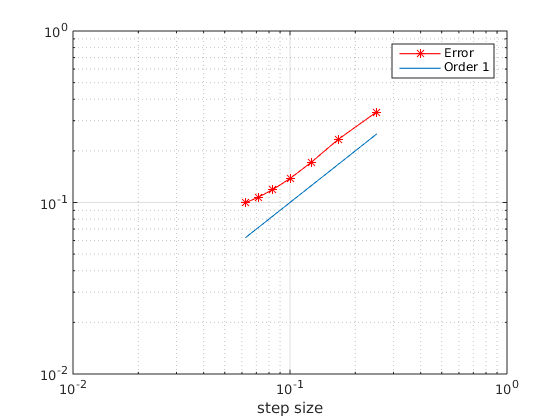
\includegraphics[width=0.4\textwidth]{convergence3d}
\caption{Logarithm error convergence plot for the 3d case, with N = 4, 6, 8, 10, 12, 14, 16 grid points in each spatial direction.}
\label{fig:convergence3d}
\end{figure}



Stress analysis
\section{Stress analysis}

The code has so far only calculated the displacement in the geometry. The stress $\bm{\sigma}$, which measures how much forces per area are acting on a particular spatial point, is very interesting when it comes to how much an object can withstand. To do a stress analysis we loop over all elements and using the relation \eqref{stress-displacement} we get the element stress vector for each element.

Of special interest is the Von Mises stress \cite{VonMises}, a scalar representation of the stress, since this can be directly compared to the materials yield strength to look for permanent displacement. The Von Mises stress is calculated as 

\begin{align*}
\sigma_{v} = \sqrt{ \frac{1}{2} \left[  (\sigma_{xx} -\sigma_{yy})^2 + (\sigma_{yy} -\sigma_{zz})^2 + (\sigma_{zz} -\sigma_{xx})^2 + 6\left(\sigma_{xy}^2 + \sigma_{yz}^2 + \sigma_{xz}^2 \right) \right]}.
\end{align*}


The Von Mises stress is saved for every element, and to get the nodal stress we average the neighboring elements. If the nodal stresses are larger then the material yield strength, we'll get a permanent deformation.


Our geometry (bridge)
Figures

Problems along the way


Conclusion, discussion



\begin{thebibliography}{2}

\bibitem{stressMatrix}
	Colorado University\\
	\emph{http://www.colorado.edu/engineering/cas/courses.d/IFEM.d/IFEM.Ch14.d/\\IFEM.Ch14.pdf}


\bibitem{stressRecovery}
	Colorado University\\
	\emph{http://www.colorado.edu/engineering/cas/courses.d/IFEM.d/IFEM.Ch28.d/\\IFEM.Ch28.pdf}	
\end{thebibliography}



\end{document}
